\chapter{Herramientas utilizadas}
\label{cap:herramientas}

Este capítulo tiene por objetivo presentar y describir las herramientas computacionales y teóricas utilizadas a lo largo de este trabajo. Específicamente, se abordará el programa \texttt{OpenMC}, la técnica estadística empleada denominada divergencia KL, los formatos de archivos usados (\texttt{MCPL} y \texttt{XML}), y los lenguajes de programación involucrados (\texttt{Python}, \texttt{C} y \texttt{C++}).

\section{\texttt{OpenMC}}

% \begin{figure}[H]
%     \centering
%     
\includegraphics[width=0.5\textwidth]{figs/openmc_logo.png}
%     \caption{Logo de \texttt{OpenMC}. Fuente: \url{https://openmc.org/}}
%     \label{fig:openmc_logo}
% \end{figure}

\texttt{OpenMC} es un programa de simulación Monte Carlo desarrollado inicialmente en el \textit{Massachusetts Institute of Technology} (\textit{MIT}) como \textit{software} de código abierto \cite{OpenMC2024}. Actualmente es mantenido por una activa comunidad internacional que contribuye continuamente a su desarrollo y expansión. Está especialmente orientado al cálculo del transporte de neutrones y fotones, permitiendo tanto simulaciones de criticidad como simulaciones de fuente fija. En este trabajo se emplean exclusivamente simulaciones de fuente fija.

Una de las ventajas de \texttt{OpenMC} es su flexibilidad en la obtención de resultados. El código permite registrar diferentes magnitudes físicas como flujos, dosis, corrientes, espectros energéticos, etc., además de ofrecer la posibilidad de registrar partículas que atraviesan superficies definidas por el usuario en un archivo de formato \texttt{h5} o \texttt{MCPL}. Estos archivos almacenan información de las variables de las partículas, permitiendo su posterior análisis o reutilización para generar nuevas simulaciones. Asimismo, \texttt{OpenMC} incorpora técnicas avanzadas de reducción de varianza, como las ventanas de peso (\textit{weight windows}), que resultan fundamentales para reducir la incertidumbre estadística de los resultados en áreas de interés específico, técnica utilizada en este trabajo.

\section{\texttt{KDSource}}

% \begin{figure}[H]
%     \centering
%     
\includegraphics[width=0.5\textwidth]{figs/kdsource_logo.png}
%     \caption{Logo de \texttt{KDSource}. Fuente: \url{https://kdsource.readthedocs.io/en/latest/}}
%     \label{fig:kdsource_logo}
% \end{figure}

\texttt{KDSource} es una herramienta computacional desarrollada en el Departamento de Física de Reactores y Radiaciones del Instituto Balseiro, cuyo objetivo principal es procesar archivos de partículas generados en simulaciones Monte Carlo para la construcción de nuevas fuentes distribucionales \cite{KDSource2024}. Su integración con \texttt{OpenMC} permite desacoplar geométricamente simulaciones complejas, facilitando significativamente el cálculo de transporte en geometrías difíciles o extensas.

El fundamento original de \texttt{KDSource} reside en la técnica \textbf{Kernel Density Estimation (KDE)}, una técnica estadística que permite estimar distribuciones continuas de variables a partir de muestras discretas, manteniendo la correlación existente entre ellas. 
% En este trabajo, se propone y desarrolla una alternativa al método KDE, utilizando histogramas multidimensionales adaptativos. Este método tiene como ventajas principales un mayor control explícito sobre la resolución local y la capacidad mejorada para capturar discontinuidades abruptas presentes en el espacio de fases.

% \texttt{KDSource} permite, además, ``rellenar huecos'' en el espacio de fases que aparecen debido a limitaciones estadísticas inherentes a los \textit{trackfiles}, lo que evita sesgos en las simulaciones posteriores y asegura una representación más completa y precisa de las distribuciones originales.

% \section{Divergencia de Kullback-Leibler (KL)}

% La divergencia KL entre distribuciones de probabilidad \( P(x) \) y \( Q(x) \) definidas sobre el mismo espacio de variables aleatorias se expresa matemáticamente como:

% \begin{equation*}
%     D_{\mathrm{KL}}(P \parallel Q) = \int_{-\infty}^{\infty} P(x) \log \left( \frac{P(x)}{Q(x)} \right) dx
% \end{equation*}

% En el caso discreto, la expresión equivalente es:

% \begin{equation*}
%     D_{\mathrm{KL}}(P \parallel Q) = \sum_{i} P(x_i) \log \left( \frac{P(x_i)}{Q(x_i)} \right)
% \end{equation*}

% % Esta es una métrica utilizada ampliamente en estadística y teoría de la información para cuantificar la distancia entre dos distribuciones de probabilidad. En este trabajo, la divergencia KL es empleada como métrica cuantitativa para evaluar la precisión del método implementado. Específicamente, se compara la similitud entre diferentes fuentes generadas a partir del mismo archivo de \textit{tracks}, permitiendo medir objetivamente el desempeño de los métodos desarrollados en términos de su capacidad para preservar correctamente las características estadísticas originales de la distribución.

% Esta es una métrica ampliamente utilizada en estadística y teoría de la información para cuantificar la distancia entre dos distribuciones de probabilidad. En este trabajo, la divergencia KL se emplea como métrica cuantitativa para evaluar la precisión de los métodos implementados. Para ello, se utiliza como referencia un \textit{trackfile} obtenido a partir de una simulación original significativamente más larga, cuya mayor estadística permite considerarlo como una buena aproximación de la distribución verdadera. La divergencia se calcula entre esta referencia y las distribuciones obtenidas a partir de fuentes remuestreadas aplicando el método desarrollado al \emph{trackfile} original, permitiendo cuantificar objetivamente la capacidad del método para preservar las características estadísticas del espacio de fases, sin verse sesgado por el ruido estadístico del \emph{trackfile} al cual se le aplicó el método.

% \section{Formato \texttt{MCPL}}

% \begin{figure}[H]
%     \centering
%     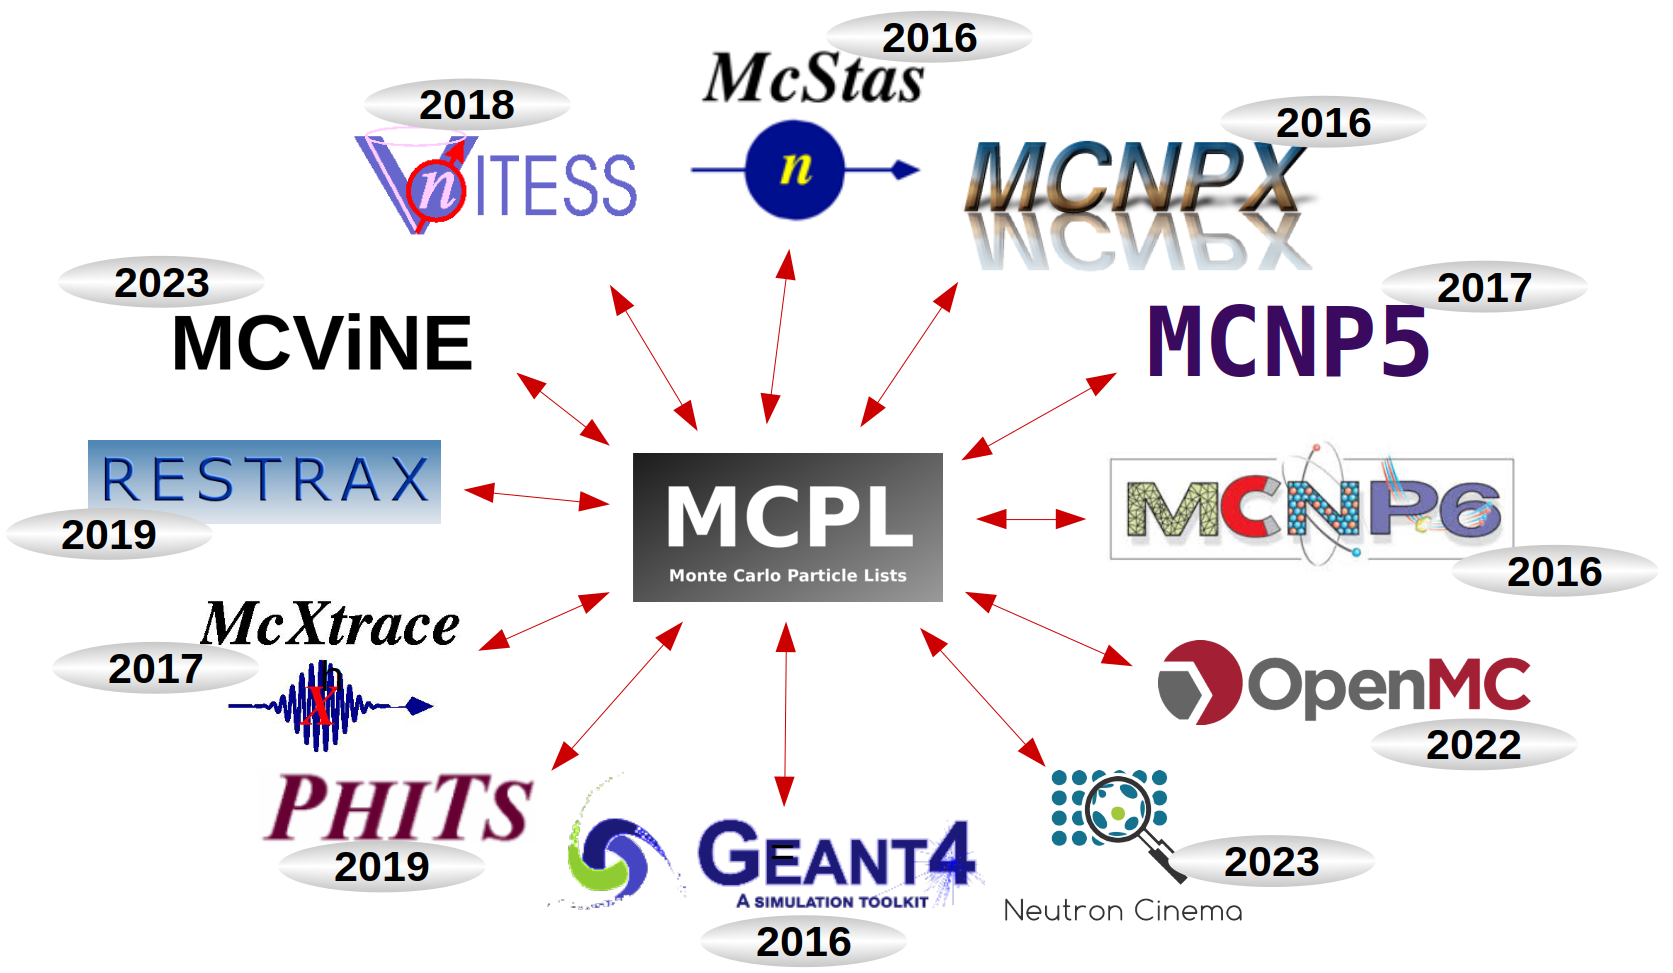
\includegraphics[width=\textwidth]{figs/mcpl_support_diagram.png}
%     \caption{Diagrama de soporte de \texttt{MCPL}. Fuente: \url{https://mctools.github.io/mcpl/}}
%     \label{fig:mcpl_support_diagram}
% \end{figure}

% El formato \textbf{\texttt{MCPL} (\textit{Monte Carlo Particle List})} es un estándar de almacenamiento de listas de particulasdesarrollado con el propósito de permitir el intercambio eficiente de información entre distintos códigos de simulación Monte Carlo. Este formato permite almacenar \textit{trackfiles} de forma eficiente y compacta, conteniendo información detallada sobre energía, posición, dirección y peso estadístico de cada partícula registrada. Su utilización en este proyecto facilita la transferencia de información entre \texttt{OpenMC}, \texttt{KDSource}, y potencialmente otros códigos de simulación.

\section{Formatos de listas de partículas: \texttt{MCPL} y \texttt{HDF5}}

En simulaciones Monte Carlo, es común registrar partículas que atraviesan una superficie o ingresan a una región de interés, generando lo que se conoce como una lista de partículas. Estos archivos permiten capturar el estado de cada partícula —incluyendo su energía, posición, dirección y peso estadístico— al momento de cruzar una superficie.

\texttt{OpenMC} emplea por defecto el formato \texttt{HDF5} para almacenar estas listas \cite{HDF5_2025}. Este formato binario jerárquico permite almacenar datos de manera eficiente, estructurada y accesible desde diversos lenguajes de programación. Sin embargo, su estructura está adaptada específicamente al ecosistema de \texttt{OpenMC}, dificultando su reutilización directa en otros códigos de transporte.

Con el objetivo de facilitar la interoperabilidad entre distintos códigos Monte Carlo, existe el formato \textbf{\texttt{MCPL} (\textit{Monte Carlo Particle List})} \cite{MCPL2024}. Este estándar de listas de partículas permite almacenar listas generadas en simulaciones de forma compacta y eficiente, preservando información esencial como la energía, posición, dirección y peso de cada partícula. A diferencia de formatos específicos como \texttt{HDF5}, \texttt{MCPL} fue concebido como una interfaz  entre diferentes entornos Monte Carlo.

La Figura \ref{fig:mcpl_support_diagram} muestra los diversos códigos que pueden producir o consumir archivos en formato \texttt{MCPL}. En este proyecto, su adopción permite vincular eficientemente los archivos de partículas generados por \texttt{OpenMC} con la herramienta \texttt{KDSource}.

\begin{figure}[H]
    \centering
    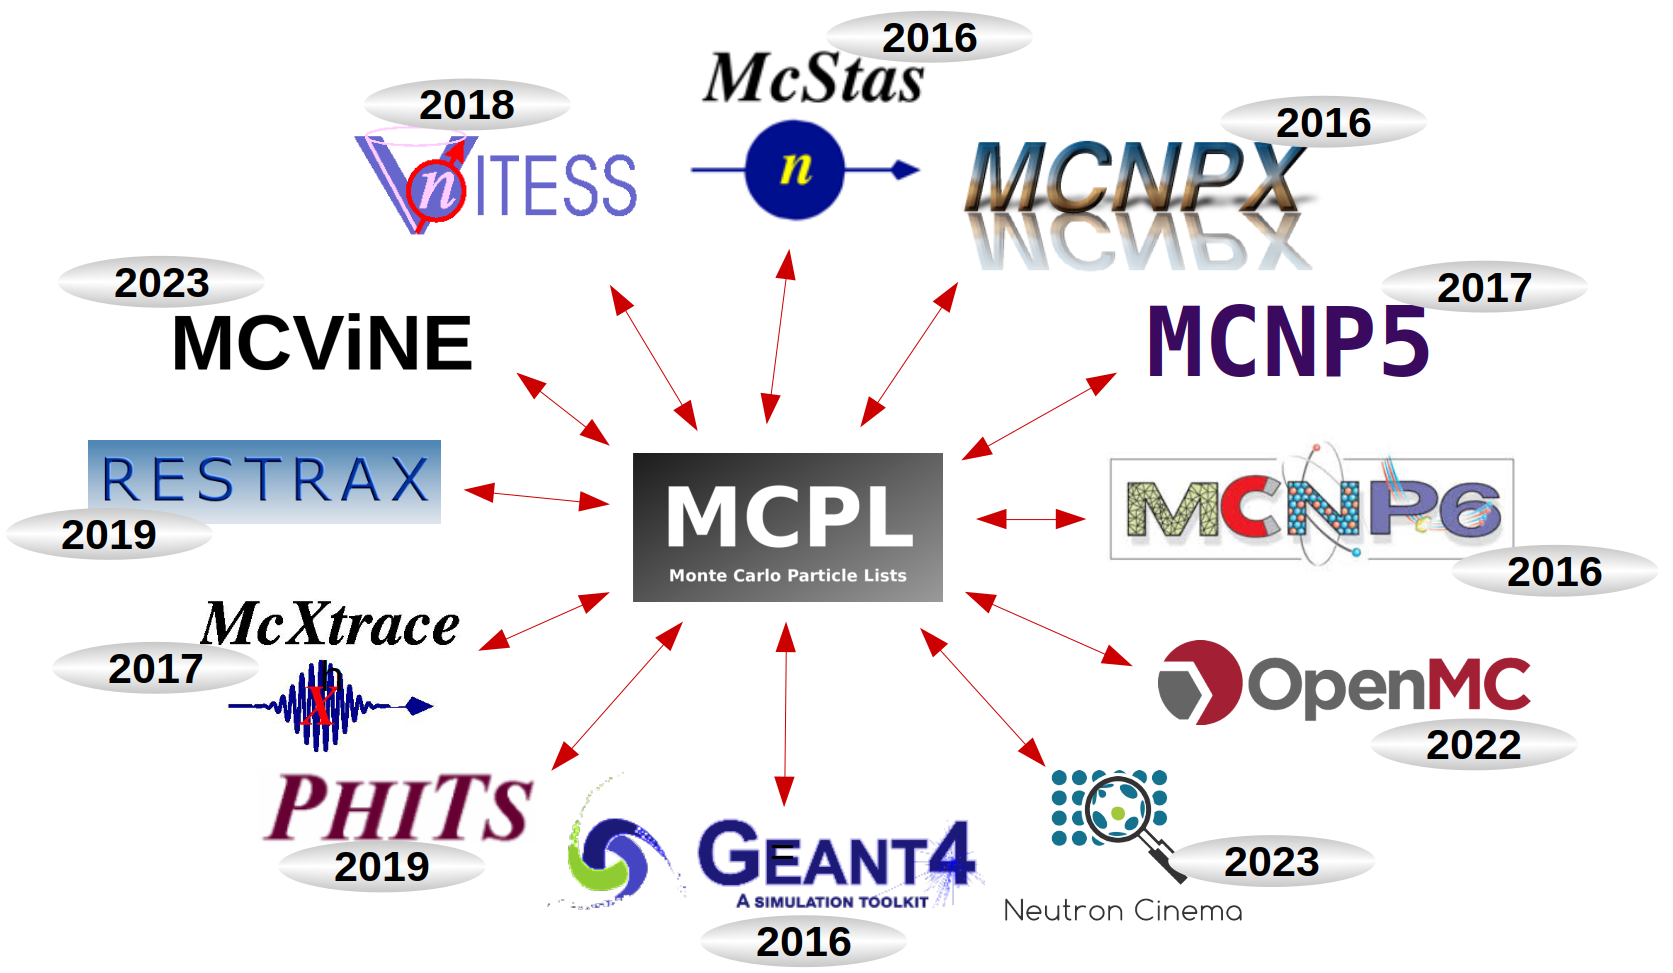
\includegraphics[width=\textwidth]{figs/mcpl_support_diagram.png}
    \caption{Diagrama de soporte de \texttt{MCPL}.}
    \label{fig:mcpl_support_diagram}
\end{figure}


\section{Formato \texttt{XML}}

% El formato \textbf{XML (Extensible Markup Language)} es un lenguaje utilizado para describir y almacenar información estructurada de manera jerárquica, basándose en una organización de datos tipo árbol. Debido a esta característica, es particularmente adecuado para guardar las distribuciones estimadas mediante histogramas multidimensionales adaptativos, método central en este trabajo. A su vez, \texttt{OpenMC} utiliza archivos XML para almacenar la configuración completa de sus simulaciones (geometría, materiales, configuración de \textit{tallies}, etc.), por lo que la elección de este formato facilita la integración entre los componentes desarrollados.

El formato \textbf{\texttt{XML} (\textit{Extensible Markup Language})} es un lenguaje utilizado para describir y almacenar información estructurada de manera jerárquica, basándose en una organización de datos tipo árbol \cite{XML2025}. Una de sus principales ventajas es que está diseñado para ser tanto legible por máquinas como por humanos, lo que facilita su edición, inspección y validación manual durante el desarrollo. Debido a estas características, resulta particularmente adecuado para guardar las distribuciones estimadas mediante histogramas multidimensionales. A su vez, \texttt{OpenMC} emplea archivos \texttt{XML} para almacenar la configuración completa de sus simulaciones (geometría, materiales, configuración de \textit{tallies}, etc.), por lo que la elección de este formato contribuye a una integración directa y eficiente entre los componentes desarrollados.

\section{Lenguajes de programación: \texttt{Python}, \texttt{C} y \texttt{C++}}

A lo largo del desarrollo del proyecto, se utilizaron principalmente tres lenguajes de programación:

% \begin{itemize}
%     \item \textbf{\texttt{Python}}: lenguaje de alto nivel especialmente adecuado para interfaces de usuario, análisis exploratorio de datos y configuración de simulaciones debido a su simplicidad, claridad y flexibilidad. \texttt{KDSource} hace uso de \texttt{Python} para la preparación y procesamiento de datos previos al muestreo Monte Carlo.

%     \item \textbf{\texttt{C}}: lenguaje de programación de bajo nivel conocido por su eficiencia computacional, velocidad y control preciso sobre la gestión de memoria. Se utilizó en este trabajo para desarrollar módulos específicos encargados del muestreo eficiente de partículas, especialmente cuando se requieren grandes volúmenes de datos.

%     \item \textbf{\texttt{C++}}: \texttt{OpenMC} está íntegramente implementado en \texttt{C++}, combinando la eficiencia de lenguajes de bajo nivel con capacidades avanzadas de abstracción y organización orientada a objetos, facilitando la integración, mantenimiento y expansión de funcionalidades del código.
% \end{itemize}

\begin{itemize}
    \item \textbf{\texttt{Python}}: lenguaje de alto nivel especialmente adecuado para interfaces de usuario, análisis exploratorio de datos y configuración de simulaciones debido a su simplicidad, claridad y flexibilidad. \texttt{KDSource} hace uso de \texttt{Python} para la preparación y procesamiento de datos previos al remuestreo Monte Carlo. Tanto \texttt{KDSource} como \texttt{OpenMC} disponen de una interfaz en Python.

    \item \textbf{\texttt{C}}: lenguaje de programación de bajo nivel conocido por su eficiencia computacional, velocidad y control preciso sobre la gestión de memoria. Se utilizó en este trabajo para desarrollar módulos específicos encargados del reuestreo eficiente de partículas, especialmente cuando se requieren grandes volúmenes de datos. La biblioteca de remuestreo de \texttt{KDSource} está escrita en este lenguaje.

    \item \textbf{\texttt{C++}}: \texttt{OpenMC} está implementado en \texttt{C++}, combinando la eficiencia de lenguajes de bajo nivel con capacidades avanzadas de abstracción y organización orientada a objetos. Esta arquitectura permite la expansión modular del código y facilita su mantenimiento.
\end{itemize}


El desarrollo realizado en este trabajo implementa un flujo computacional para el uso de fuentes distribucionales en simulaciones Monte Carlo. Este flujo se compone de tres etapas principales: detección, procesamiento y producción, y aprovecha las capacidades de los lenguajes \texttt{Python}, \texttt{C} y \texttt{C++}.

\textbf{Detección}: se realiza mediante una simulación inicial en \texttt{OpenMC}, en la cual se registra un archivo de partículas sobre una superficie. Este archivo puede guardarse en formato \texttt{HDF5}, que es el formato nativo de \texttt{OpenMC}, y luego ser convertido al formato \texttt{MCPL} si se desea continuar con el procesamiento. Alternativamente, si \texttt{OpenMC} fue compilado con soporte para \texttt{MCPL}, puede generarse directamente en dicho formato. El archivo resultante se almacena en disco para su uso posterior. Este procedimiento se ilustra en la Figura \ref{fig:flujo_deteccion}.

\begin{figure}[H]
    \centering
    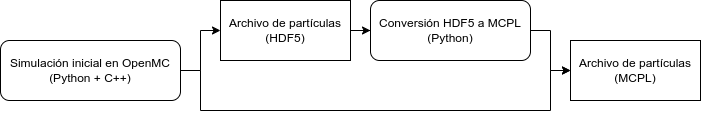
\includegraphics[width=0.75\textwidth]{flujo_codigos-Deteccion.png}
    \caption{Etapa de detección: registro de partículas en formato \texttt{MCPL} a partir de una simulación en \texttt{OpenMC}.}
    \label{fig:flujo_deteccion}
\end{figure}

\textbf{Procesamiento}: esta etapa se lleva a cabo en \texttt{Python} utilizando la implementación desarrollada para procesar mediante histogramas multidimensionales. A partir del archivo \texttt{.MCPL}, se construye una fuente distribucional que representa la densidad de probabilidad estimada en el espacio de fases. El resultado de esta etapa es un archivo \texttt{XML}, que contiene la parametrización de la fuente y se almacena en disco como entrada para la etapa de producción. La Figura \ref{fig:flujo_procesamiento} muestra un esquema de esta etapa.

\begin{figure}[H]
    \centering
    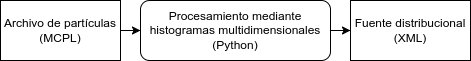
\includegraphics[width=0.55\textwidth]{flujo_codigos-Procesamiento.png}
    \caption{Etapa de procesamiento: construcción de una fuente distribucional a partir de un archivo \texttt{MCPL}.}
    \label{fig:flujo_procesamiento}
\end{figure}

\textbf{Producción}: esta etapa puede abordarse de dos maneras, implementada en código \texttt{C}. En la modalidad \textit{offline}, el archivo \texttt{XML} es utilizado para generar una nueva lista de partículas en formato \texttt{MCPL}, que luego puede emplearse directamente como fuente en \texttt{OpenMC} si se cuenta con soporte para este formato. En caso contrario, puede convertirse nuevamente a \texttt{HDF5}. En la modalidad \textit{on-the-fly}, se evita por completo el uso de listas intermedias: \texttt{OpenMC} accede directamente al archivo \texttt{XML} y realiza el remuestreo dinámicamente durante la simulación, gracias a una extensión \emph{ad-hoc} incorporada en este trabajo. Ambas modalidades se ilustran en la Figura \ref{fig:flujo_produccion}.

\begin{figure}[H]
    \centering
    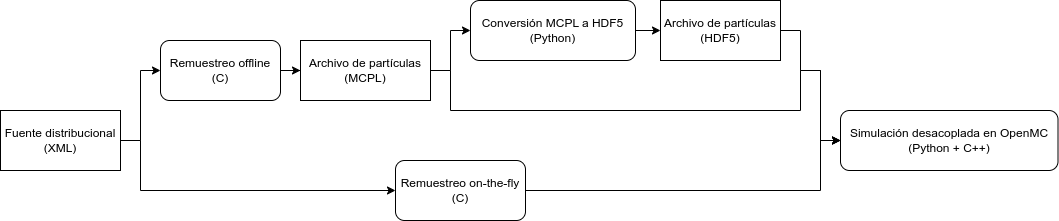
\includegraphics[width=\textwidth]{flujo_codigos-Remuestreo.png}
    \caption{Etapa de producción: uso del archivo \texttt{XML} para generar nuevas partículas de forma offline o on-the-fly.}
    \label{fig:flujo_produccion}
\end{figure}

En las Figuras \ref{fig:flujo_deteccion}, \ref{fig:flujo_procesamiento} y \ref{fig:flujo_produccion}, los bloques con esquinas redondeadas representan procesos computacionales, mientras que los bloques rectangulares indican archivos que se registran o leen desde disco.


